\documentclass{article}

\usepackage[UTF8]{ctex}
\usepackage[a4paper, total={6.8in,9.2in}]{geometry}
\usepackage{abstract}
\usepackage{lmodern}
\usepackage{cite}
\usepackage{float}
\usepackage{booktabs}
\usepackage{tabularx}
\usepackage{longtable}
\usepackage{multicol}
\usepackage{hyperref}
\usepackage{amsmath}
\usepackage{dirtree}
\usepackage{authblk}
\usepackage{tikz}
\usetikzlibrary{graphs, positioning, quotes, shapes.geometric}

\hypersetup{hidelinks,
    colorlinks=true,
    allcolors=black,
    pdfstartview=Fit,
    breaklinks=true}

\renewcommand*{\Authsep}{, }
\renewcommand*{\Authand}{, }
\renewcommand*{\Authands}{, }

\begin{document}

\title{一种基于人工智能技术的系统发生树绘制与物种演化路径推断系统}
\author[a]{朱璟瑞\thanks{通讯作者: 870239526@qq.com}}
\author[a]{胡高远}
\author[a]{邓钰潼}
\affil[a]{河南科技大学附属高级中学(周山校区), 471031}
\date{\today}
\maketitle

\begin{abstract}
    \par
    近些年来,随着分子生物学的发展,基因序列与蛋白质序列越来越多地被作为绘制系统发生树的重要参考依据,从中诞生了很多相应的技术。
    但是,这些技术在实践过程中,仍存在着一些问题。比如参考序列选择比较困难等,这些都给绘制出的系统发生树的准确性与严谨性带来了一定的影响。
    在本文中,笔者搭建了一套用于绘制系统发生树的计算机应用软件,这套系统集成了一些常用的比对与建树算法,同时,该系统还综合了近期的相关科研数据,
    使用了人工智能(AI)技术以对建成的系统发生树进行综合分析,从而得出最优异的、最能代表真实物种演化路径的系统发生树,
    这一突破,能够使得研究人员无需拘泥于参考序列的选择,可缩短科研周期,提升科研效率。
    同时,本系统包括了插件系统,这使得用户可以自定义需要的序列比对与建树算法,可扩展性更强。
    该系统的综合能力优于目前市面上的几款解决方案,使物种演化路径的推断过程变得更加便利、准确,对相关的科研工作可能会起到推进作用。
    \par\textbf{关键词: } 分子生物学, 序列比对, 系统发生树, 计算机应用软件, 人工智能
\end{abstract}

\pagenumbering{roman}
\tableofcontents
\newpage
\pagenumbering{arabic}

\begin{multicols}{2}

\section{序列比对与系统发生树构建的相关算法简介}
\par
作为一种物种演化路径推断系统,序列比对算法与系统发生树构建算法自然是重中之重,下面笔者将介绍本系统中所使用的几种相关算法:

\subsection{序列比对方法}
\par
序列比对是将两个或多个核酸序列或蛋白质序列排列在一起,以揭示它们之间的相似性和差异性的过程。
本系统的序列比对过程,采用的是 Needleman-Wunsch 算法,这一算法效率高、准确性好,是目前业内最常用的序列比对算法之一。

\subsubsection{Needleman-Wunsch算法}
\par
Needleman-Wunsch算法是将动态规划算法应用于生物序列的比较的最早期的几个实例之一。该算法是由 Saul B. Needlman 和 Christian D. Wunsch 两位科学家于1970年发明的\cite{ref2}。
该算法的状态转移方程如下:

\begin{equation}
\begin{aligned}
F(0,0) &= 0 \\
F(i,j) &= \max \left\{
      \begin{array}{lr}
      F(i-1,j-1) + s(x_i,y_j) &  \\
      F(i-1,j)+d & \\
      F(i,j-1)+d &
      \end{array}
\right.
\nonumber
\end{aligned}
\end{equation}

\par
在生物序列比对算法中,该算法拥有很多优良的特性,如准确度较高、适用于多种序列的比对等。故本项目使用的默认算法便是本算法。

\subsection{系统发生树构建方法}
\par
常见的系统发生树构建方法有很多,比如最小进化法、最大似然法等等。受开发时间限制,本系统只自带了非加权组平均法与邻接法的建树算法。
关于其他方法,用户可以通过本系统的插件系统自行添加。

\subsubsection{非加权组平均法}
\par
非加权组平均法(UPGMA,unweighted pair-group method with arithmetic means)是一种常用的聚类分析方法。
其算法思想基于聚类分析,其核心在于通过计算不同对象之间的距离来确定它们之间的亲缘关系\cite{ref3}。
其具体的算法流程分为以下三步:
\par
首先,需要计算所有对象(如物种、基因序列等)之间的距离。
\par
找出距离最小的两个对象(OTU,Operational Taxonomic Units,操作分类单元),将它们聚为一个新的OTU。
新的OTU的分支点位于这两个OTU间距离的1/2处。计算新的OTU与其他OTU之间的平均距离。
重复上述步骤,找出距离最小的两个OTU(可以是原始的OTU或之前聚类形成的新OTU)进行聚类。
如此反复,直到所有的OTU都聚到一起,形成一个完整的系统发生树。
\par
通过上述聚类过程,最终可以得到一个表示物种间亲缘关系的系统发生树。
在系统发生树中,每个节点代表一个OTU,节点之间的连线表示它们之间的亲缘关系,连线的长度则反映了它们之间的进化距离。

\subsubsection{邻接法}
\par
邻接法(Neighbor-Joining,NJ)是由Naruya Saitou和Masatoshi Nei于1987年首次提出的一种用于构建系统发育树的聚类方法\cite{ref5}。
邻接法的算法思想基于最小进化原理,即在整个进化过程中,树的分支长度之和达到最小。
该算法从一个完全未解析的树开始,然后通过迭代过程逐步构建出完整的系统发育树。具体算法流程如下:
\par
初始化一个完全未解析的树,其拓扑结构对应于星形网络,所有分类单元都从一个中心节点出发。
\par
在每一步迭代中,基于当前的距离矩阵计算一个称为Q的矩阵。Q矩阵的元素Q(i,j)表示将分类单元i和j连接到一个新的中间节点时,树的分支长度之和的增加量。
在Q矩阵中找到最小值Q(i,j),将对应的分类单元i和j连接到一个新的中间节点u。计算每个分类单元到新节点u的距离,并更新距离矩阵。
迭代上述过程,用新节点替换连接的邻居对,并使用前一步计算的距离更新距离矩阵。
\par
当所有分类单元都被合并到树中,且树的拓扑结构完全解析时,迭代过程终止。

\subsection{常见的解决方案及其弊端}
\par
系统发生树构建与物种演化路径推断,现如今市面上已经有了几种常见的解决方案,但它们都有各自的弊端。
\par
其中,单独进行某一环节的工具,如用于序列比对的Clustal X, MAFFT等\cite{ref1},虽然在该环节上拥有良好的性能,但并不能支持从序列到系统发生树的全过程,
这使得研究人员需要频繁周转于多个平台,增加了研究需要的时间。
\par
而一些支持全环节的工具,如MEGA等,能够支撑整个科研流程,但它们的可扩展性往往不佳,无法支持用户更加多元化的需求。
\par
同时,由系统发生树得出生物演化路径,仍然需要较长的研究时间。因为并非基于所有同源序列绘制出的系统发生树,都是可以代表生物演化的路径的。
而研究人员往往需要从繁杂的系统发生树数据中,找到能够提示真实生物演化路径的树,在某些研究中,这一过程相当繁杂,这无疑为科研人员的研究带来了诸多不便

\section{本系统的基础架构}
\par
本系统是支持从序列解析到系统发生树渲染的,全流程的综合平台,本系统“从序列到树”的流程如下:

\begin{tikzpicture}[node distance=10pt]
    \node[draw, rounded corners]                        (start)   {Start};
    \node[draw, below=of start]                         (step 1)  {序列识别};
    \node[draw, below=of step 1]                        (step 2)  {序列比对};
    \node[draw, below=of step 2]                        (step 3)  {建树};
    \node[draw, below=of step 3]                        (step 4)  {渲染成图};
    \node[draw, right=30pt of step 3]                   (step 5)  {AI修正};
    \node[draw, rounded corners, below=of step 4]       (end)     {End};

    \graph{
    (start) -> (step 1) -> (step 2) -> (step 3) -> (step 4) -> (end);
    (step 3) -> (step 5);
    (step 5) -> (step 3);
    };
\end{tikzpicture}

\par
作为一款计算机软件,本系统主要采用了Python作为编码语言。
\par
Python由荷兰国家数学与计算机科学研究中心的 Guido van Rossum 于1990年代初设计\cite{ref4}。Python提供了高效的高级数据结构,还能简单有效地面向对象编程。
Python语法和动态类型,以及解释型语言的本质,使它成为多数平台上写脚本和快速开发应用的编程语言,随着版本的不断更新和语言新功能的添加,逐渐被用于独立的、大型项目的开发。
基于Python的许多优良的特性以及其良好的可扩展性、丰富的社区内容,我们决定使用Python构建本系统。
\par
本系统的软件架构(除数据外)共分为三个部分:算法包、用户系统、插件系统。本系统的软件目录树(源代码)如下:
\par
% \makeatother
\dirtree{%
.1 AITD System.
.2 aitd\DTcomment{aitd 算法包}.
.3 {\_\_init\_\_.py}\DTcomment{主文件}.
.3 {error.py}\DTcomment{错误类文件}.
.3 {xlist.py}\DTcomment{算法目录文件}.
.2 data\DTcomment{软件数据}.
.3 fonts\DTcomment{字体文件夹}.
.4 {...}.
.3 icons\DTcomment{图标文件夹}.
.4 {...}.
.3 {setting.dat}\DTcomment{软件设置数据}.
.3 {en.yml}\DTcomment{语言数据(英文)}.
.3 {zh\_CN.yml}\DTcomment{语言数据(中文简体)}.
.2 licenses\DTcomment{许可证文件夹}.
.3 {...}.
.2 plugins\DTcomment{插件文件夹}.
.3 xxx\DTcomment{安装的某一个插件}.
.4 {...}.
.3 {plugin\_list.json}\DTcomment{已安装的插件目录}.
.2 {aitd\_c.py}\DTcomment{命令提示符端}.
.2 {aitd\_w.pyw}\DTcomment{窗口端}.
.2 {LICENSE}\DTcomment{开源许可证}.
}

\subsection{算法嵌入、项目文件夹及命名空间系统}

\subsubsection{算法嵌入}
\par
本系统自带的序列比对、系统发生树构建等算法的源代码均在 \verb|aitd\__init__.py| 中。
所有算法(除人工智能外)被分为以下五种:

\begin{itemize}
\item[1)] 文件解析器(Parser):解析序列文件格式并存储序列信息;
\item[2)] 序列比对(Comparator):比对两个或多个序列;
\item[3)] 比对加载(Processor):根据比对结果判断两个序列的差异性;
\item[4)] 建树(TreePlanter):根据多个序列之间的差异性绘制系统发生树;
\item[5)] 草图绘制(Display):将系统发生树绘制成图像。
\end{itemize}

\par
算法实装时,使用 \verb|setattr| 函数将该算法的执行函数设置为 \verb|aitd.xlist| 中对应的列表实例的成员函数,同时给算法赋予一个名字。
当需要使用该种算法时,可直接使用 \verb|getattr| 函数获取对应名字的成员函数。

\subsubsection{项目文件夹}
\par
本系统会将用户的数据存储为自定义的项目文件夹。项目文件夹的目录如下:
\par
\dirtree{%
.1 {<项目名>}.
.2 cache\DTcomment{缓存文件夹}.
.3 log\DTcomment{运行日志}.
.4 {...}.
.3 sketch\DTcomment{建树草图}.
.4 {...}.
.3 {...}.
.2 data\DTcomment{数据文件夹}.
.3 sequence\DTcomment{序列数据}.
.4 {.seq}\DTcomment{序列内容}.
.4 {.metadata}\DTcomment{序列元数据}.
.4 {...}.
.3 alignment\DTcomment{对比结果}.
.4 {.ali}\DTcomment{序列对比结果}.
.4 {.ali.dat}\DTcomment{对比得分数据}.
.4 {...}.
.3 tree\DTcomment{系统发生树}.
.4 {.tree}\DTcomment{系统发生树文件}.
.4 {...}.
.3 correction\DTcomment{AI修正结果}.
.4 {...}.
.2 training\DTcomment{AI训练文件夹}.
.3 {...}.
.2 {setting.dat}\DTcomment{项目设置}.
.2 {setting.json}\DTcomment{命名空间}.
}
\par
其中, \verb|setting.json| 内提供了本项目内所有数据的命名空间名、文件地址、格式等基本信息,是向系统表示该项目属性的重要依据。


\subsubsection{命名空间系统}
\par
本系统中的所有数据(算法,项目数据等)在软件运行时,均会被赋予一个唯一确定的名字,即命名空间名(Name in the namespace),以便于进行定位与引用。
每一个命名空间名由数据类型和名称标识两部分构成,两部分之间由两个半角冒号(\verb|::|)连接。
\par
在打开某一个项目后,系统会首先读取项目文件夹中的 \verb|setting.json| 文件,这个文件中存储了所有项目数据的命名空间名以及项目文件的存储地址。
随后,系统会将这些数据,以及系统自带的算法等数据全部存储进 \verb|namespace : dict| 中。
\par
命名空间系统中的所有命名空间列表如下:
\par
\begin{table}[H]
\caption{\textbf{命名空间表}}
\centering
\begin{tabular}{cc}
\toprule
命名空间&存储的内容\\
\midrule
seq::&序列数据\\
ali::&比对结果数据\\
tree::&系统发生树数据\\
sketch::&草图数据\\
ParserList::&序列文件解析器\\
ComparatorList::&序列比对器\\
MatrixList::&序列比对用矩阵\\
TreePlanterList::&建树算法\\
DisplayList::&草图渲染器\\
ModelList::&AI模型\\
\bottomrule
\end{tabular}
\end{table}
% \lstinputlisting[
%     style       =   Python,
%     caption     =   {},
%     label       =   {code:1}
% ]{./code1.py}

\subsection{基于Python的控制台+窗体化双端系统}
\par
本系统的用户系统分为控制台端和窗口端双端,用户可以自行选择使用控制台或窗口进行工作。
\subsubsection{窗体端}
\par
其中,本系统的窗口端使用tkinter为窗体化的基本框架,并使用matplotlib作为图表渲染的工具。
本系统窗口段的用户界面共分为三部分:菜单栏、侧栏、主栏。这四部分的标示如下图所示。
\par
\begin{figure}[H]
\centering
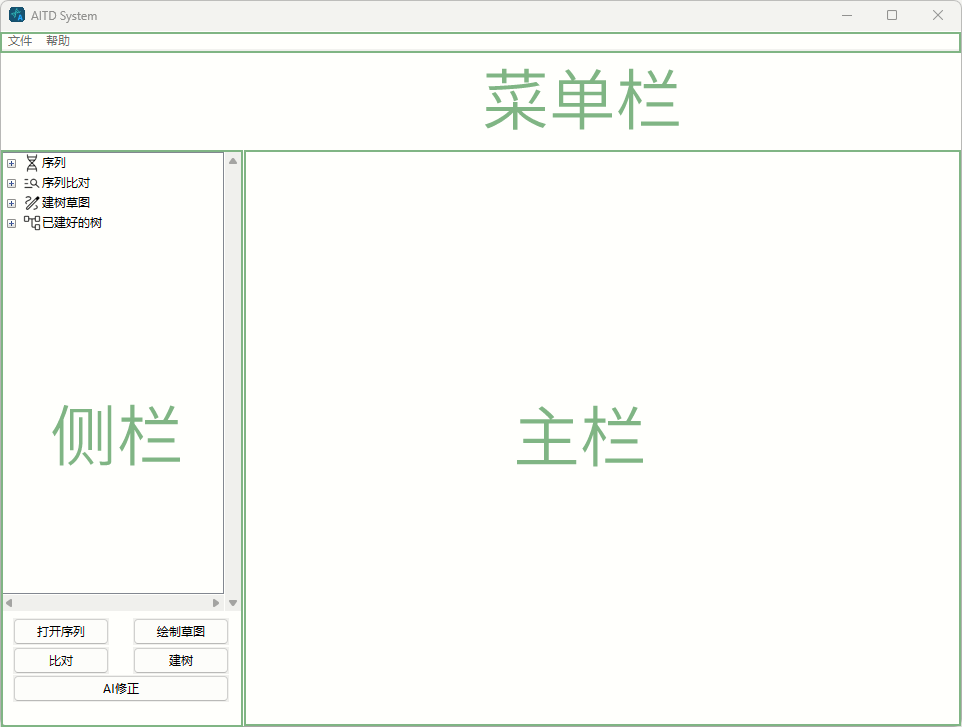
\includegraphics[width=0.4\textwidth]{A.png}
\caption{用户界面分栏示意}
\end{figure}
\par
当打开了某个项目后,侧栏会出现项目内的数据文件表、同时提供了一些操作(如序列导入、序列比对、建树后)。
当选择了某种操作后,主栏会出现该操作的各种配置项。比如下图便展示了“序列查看”操作的配置项(图中所打开的是 Escherichia coli str. K-12 细胞色素C基因的序列,序列来源:NCBI)。
\par
\begin{figure}[H]
\centering
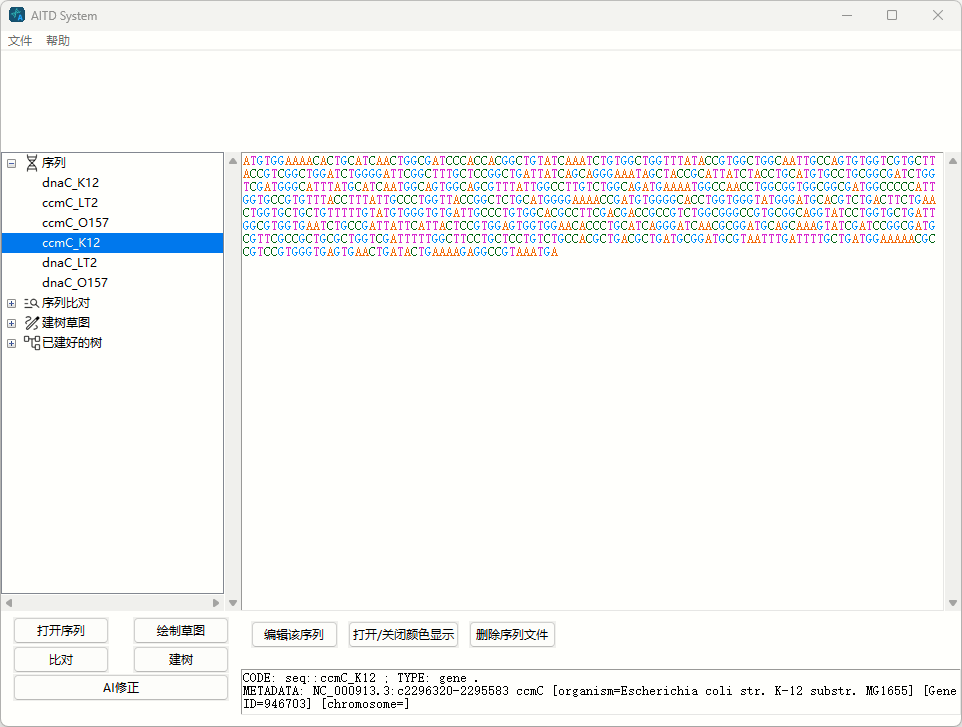
\includegraphics[width=0.4\textwidth]{B.png}
\caption{“序列查看”操作}
\end{figure}
\subsubsection{控制台端}
\par
对于控制台端,本系统同样使用matplotlib作为图表渲染工具.
本系统控制台端主要分为三个模式: Normal Mode. Debug Mode, Project Mode.
\par
其中,在Normal Mode中,用户可以对控制台端的默认设置进行更改等操作。
Project Mode中, 用户可以对当前的项目进行操作,包括导入序列,对比序列,导出生成的数据等
Debug Mode可以在上述两个模式的基础的同时,允许用户执行单行python代码以方便用户对控制台端程序进行调试。

\section{人工智能的引入}

\subsection{人工智能模型的设计}

\subsection{训练用数据的来源}
\par
为了使人工智能输出的结果尽量正确,我们决定选择近几年的几个涵盖物种树较广的研究作为训练用数据的来源。
Joseph N Keating等在2023年使用了多个已发表的,包括形态学和分子数据的数据集,构建系统发育树,并评估形态学和分子数据之间的不一致性\cite{ref6};
Alexandre R. Zuntini等在2024年通过对大量被子植物的基因组序列数据进行分析,揭示了被子植物在进化历史上的多样化和特定谱系的历史\cite{ref7}。
Upham NS等在2019年利用6000多种现存的哺乳动物,使用贝叶斯方法构建了系统生成树,刻画了它们之间的演化关系\cite{ref8}。
这两个研究提供了足够多的训练人工智能模型的数据,我们使用这些数据进行训练。

\subsection{训练过程}


\section{本系统的测试与展望}

\subsection{系统的可扩展性与可移植性}

\subsubsection{可扩展性}
\par
本系统开发了插件系统(Plug-in System),这使得用户可以根据自己的需求,编写插件使得本系统支持更多的功能。目前,本系统暂时只支持使用Python编写插件。
\par
一个可以被本系统识别的插件应至少有一个 \verb|setting.json| ,用以向系统表明该插件的属性。
\par
一个完整的 \verb|setting.json| 由四部分组成。第一部分是插件的基本信息(名称,作者信息等);第二部分是插件的配置项;
第三部分负责向系统表明当系统运行到特殊时刻(系统启动、窗口被刷新等)时插件会执行哪些代码;第四部分负责添加该插件内包含的算法。
\par
同时,为了方便插件与系统进行数据交流,第三与第四部分还可以添加 \verb|args| 参数。系统可以以这些参数为接口,向插件传递信息,以及一些系统自带的函数。
\par
这一套插件系统的引入,极大地增加了系统的可扩展性,使得研究人员能够最大程度地改造系统以利于科研。

\subsubsection{可移植性}
\par
本系统基于Python开发,这一语言本身就拥有者跨平台的优点。同时,本系统所使用的第三方库也均经过了筛选,绝大多数都有着良好的可移植性。
这些特点使得本系统在多种平台上预计均有着良好的兼容性。

\subsection{系统对物种演化路径的准确判断及其便利性}

\subsection{目前存在的问题}
\par
由于从提出设想到付诸实现只经过了不到一个月的周期,本项目的很多地方还没有打磨完善,至今仍存在部分问题。
\par
\begin{itemize}
\item[1)] 受开发时间限制,本项目的算法包中只包含了少数几种算法;
\item[2)] 由于训练用数据量尚且不足,AI系统输出的结果可能有一定的偏差;
\item[3)] 尚未对项目进行系统性的鲁棒性测试,这可能导致运行过程中出现一些不可预知的错误。
\end{itemize}
\par
但同时,这一系统也已经达到了我们在如此短的时间内能够达到的最好的效果。
今后,我们会进一步增加算法包中的算法数目,扩展训练数据,进一步提升本系统的综合能力。

\subsection{项目地址}
\par
本项目的所有源码与数据均基于 Apache 2.0 License 开源。
本项目的github仓库地址:\href{https://github.com/ruufly/AITD-System}{https://github.com/ruufly/AITD-System}。
本项目发布版会随后续开发进度发布在github仓库中。

\section{致谢与作者贡献声明}

\subsection{作者贡献声明}
\par
朱璟瑞(第一作者):项目的发起者,完成了项目整体框架的构建、窗口端与算法库的代码;
\par
胡高远:负责了人工智能模型的构建;
\par
邓钰潼:主导了人工智能训练用数据的寻找,完成了控制台端的代码;

\subsection{致谢}
\par
感谢洛阳外国语学校(杨湾校区)的白致远,他提供了训练人工智能所必需的算力资源。
\par
感谢华东师范大学计算机科学与技术学院的赵静博士,她为本项目人工智能模型的构建提了很多建设性的意见;
% \par
% 感谢马来西亚国立大学的刘东升,他帮助我们进行了提示文本与项目文档的英文翻译的审校工作;
\par
感谢河南科技大学附属高级中学的常易凡老师、陈洪武老师、朱晓东老师,作为我们的指导老师,他们为本项目的构建提供了一些帮助;
\par
感谢河南科技大学附属高级中学的张剑辉老师、罗会杰老师,他们带领笔者走进了生物学和信息技术的大门,本项目的构建亦有他们间接的帮助;
\par
谨以此项目献给河南科技大学附属高级中学的张丹丹老师,感谢您这两年对我们的谆谆教诲,祝愿您生下一个健康快乐的宝宝!

\bibliographystyle{IEEEtran}
\bibliography{IEEEexample}
\begingroup
\renewcommand{\section}[2]{}
\begin{thebibliography}{100}
    \bibitem{ref1} 彭焕文, 王伟. 基于分子数据的系统发生树构建[J]. 植物学报, 2023, 58(02): 261-273.
    \bibitem{ref2} Needleman SB, Wunsch CD. A general method applicable to the search for similarities in the amino acid sequence of two proteins[J]. J Mol Biol, 1970 Mar, 48(3): 443-53.
    \bibitem{ref3} mmqwqf. 基于python的非加权分组平均法构造简单系统发生树(DNA)[EB/OL]. (2020-10-12), https://blog.csdn.net/mmqwqf/article\newline/details/108988456..
    \bibitem{ref4} Python Software Foundation. History and License[EB/OL]. (2024-09-21), https://docs.python.org/3/license.html.
    \bibitem{ref5} Saitou N, Nei M. The neighbor-joining method: a new method for reconstructing phylogenetic trees[J]. Mol Biol Evol. 1987 Jul; 4(4):406-25.
    \bibitem{ref6} Keating, J.N., Garwood, R.J. and Sansom, R.S. Phylogenetic congruence, conflict and consilience between molecular and morphological data[J]. BMC Ecol Evo 23, 30 (2023).
    \bibitem{ref7} Zuntini, A.R., Carruthers, T., Maurin, O. et al. Phylogenomics and the rise of the angiosperms[J]. Nature 629, 843–850 (2024).
    \bibitem{ref8} Upham NS, Esselstyn JA, Jetz W. Inferring the mammal tree: Species-level sets of phylogenies for questions in ecology, evolution, and conservation[J]. PLoS Biol. 2019 Dec 4;17(12):e3000494.
\end{thebibliography}
\endgroup
\end{multicols}

\end{document}